\documentclass[11pt,a4paper]{article}
\usepackage{fullpage}
\usepackage[T1]{fontenc} 
\usepackage[utf8]{inputenc}
\usepackage{amsmath}
\usepackage{amssymb}
\usepackage{amsthm}
\usepackage{float}
\usepackage{tabularx}
\usepackage{graphicx}
\usepackage[hidelinks]{hyperref}
\usepackage[polish]{babel}

\DeclareMathOperator{\Initially}{\textbf{\textit{initially}}}
\DeclareMathOperator{\After}{\textbf{\textit{after}}}
\DeclareMathOperator{\Observable}{\textbf{\textit{observable}}}
\DeclareMathOperator{\Causes}{\textbf{\textit{causes}}}
\DeclareMathOperator{\If}{\textbf{\textit{if}}}
\DeclareMathOperator{\Impossible}{\textbf{\textit{impossible}}}
\DeclareMathOperator{\Releases}{\textbf{\textit{releases}}}
\DeclareMathOperator{\Always}{\textbf{\textit{always}}}
\DeclareMathOperator{\Sometimes}{\textbf{\textit{sometimes}}}
\DeclareMathOperator{\Noninertial}{\textbf{\textit{noninertial}}}

\DeclareMathOperator{\Executable}{\textbf{\textit{executable}}}
\DeclareMathOperator{\Accessible}{\textbf{\textit{accessible}}}
\DeclareMathOperator{\Possibly}{\textbf{\textit{possibly}}}
\DeclareMathOperator{\Necessary}{\textbf{\textit{necessary}}}


\setlength{\parindent}{0cm}
\setlength{\parskip}{2mm}
\begin{document}

\title{Reprezentacja wiedzy \\
\Large{
    Projekt nr~4 --- Programy działań z akcjami współbieżnymi \\
    Raport z~implementacji i~testów
}}
\author{
    Bartłomiej Dach (szef) \and
    Jacek Dziwulski \and
    Tymon Felski \and
    Jędrzej Fijałkowski \and
    Filip Grajek \and
    Maciej Grzeszczak \and
    Michał Kołodziej \and
    Piotr Piwowarski \and
    Mateusz Rymuszka \and
    Piotr Wolski
}
\maketitle

Niniejszy dokument zawiera raport z~implementacji projektu dotyczącego akcji współbieżnych wraz z~instrukcją obsługi stworzonego programu.
Ponadto w~dokumencie zawarty jest raport z~fazy testów, podział prac w~grupie oraz~lista zawartości dołączonej płyty~CD.

\section{Instrukcja obsługi}

Do~wprowadzania zdań języka akcji oraz~kwerend opracowane zostały dwa~warianty interfejsu użytkownika:
\begin{itemize}
    \item Pierwszy wariant, dostępny w~zakładce \emph{Edycja}, to~typowy edytor graficzny, podobny działaniem do~edytora równań w~programach pakietu biurowego Microsoft Office.
    W~tym wariancie zdania konstruowane~są poprzez~zaznaczanie odpowiednich elementów w~oknach edycji i~użycie opcji na~górze okna w~celu wypełnienia zdań zgodnie z~życzeniem użytkownika.
    \item Drugą opcją jest zwykły edytor tekstowy, dostępny w~zakładce \emph{Gramatyka}.
    W~tym wariancie formuły wprowadzane są w~postaci tekstowej i~interpretowane z~użyciem stworzonej gramatyki bezkontekstowej, która konwertuje zapis zdań na~ich postać semantyczną.
\end{itemize}
Oba rodzaje edytorów opisane są szerzej w~poniższych podrozdziałach.

\subsection{Edytor graficzny}

\begin{figure}[H]
    \centering
    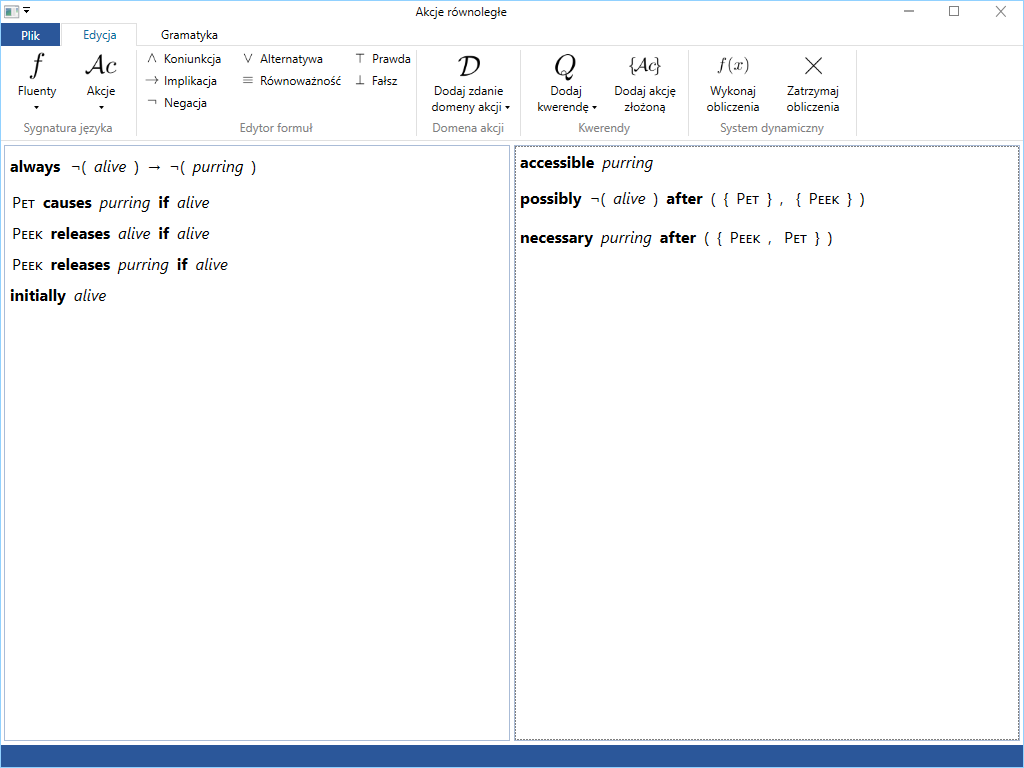
\includegraphics[width=0.8\textwidth]{res/img/visual-editor.png}
    \label{fig:visual-editor}
    \caption{Wygląd edytora graficznego}
\end{figure}

\subsection{Edytor tekstowy}

\begin{figure}[H]
    \centering
    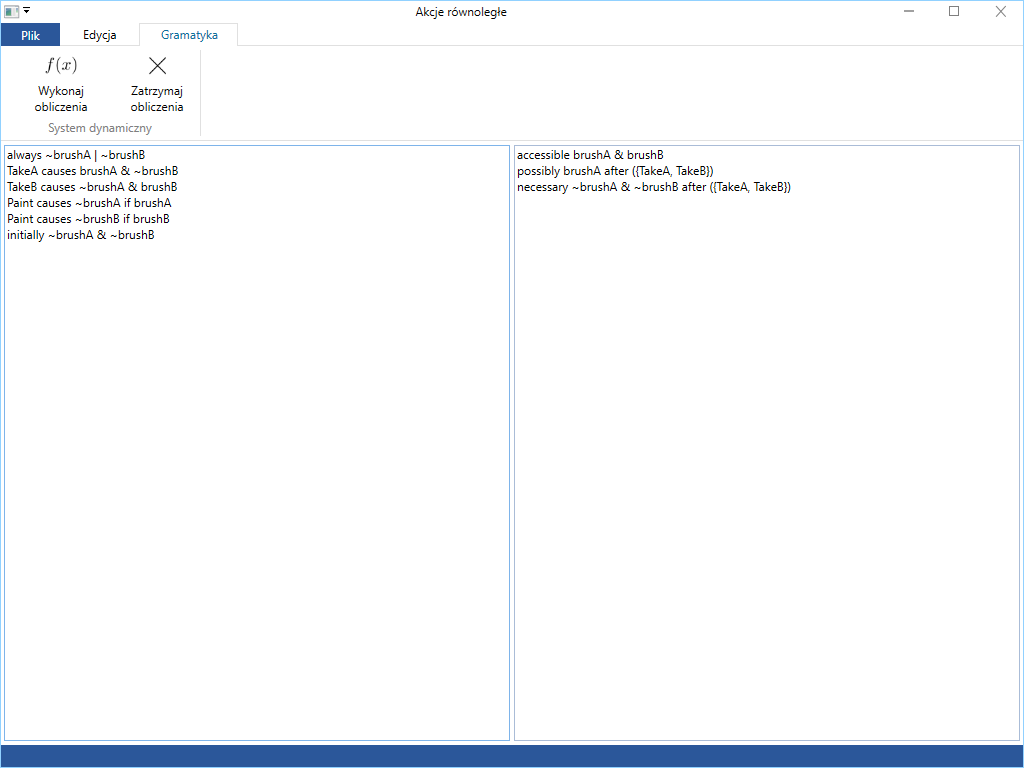
\includegraphics[width=0.8\textwidth]{res/img/grammar-editor.png}
    \label{fig:grammar-editor}
    \caption{Wygląd edytora tekstowego}
\end{figure}

Edytor tekstowy stanowi uproszczoną metodę wprowadzania scenariusza do~programu.
W~tym wariancie okno programu składa~się z~dwóch pól tekstowych:
\begin{itemize}
    \item Lewe pole tekstowe służy do~wprowadzania zdań języka akcji.
    \item Prawe pole tekstowe służy do~wprowadzania zdań języka kwerend.
\end{itemize}
Składnia wprowadzanych zdań jest zgodna z~tą wyspecyfikowaną w~dokumentacji teoretycznej.
Jedyną różnicą jest wprowadzanie formuł --- dla~wygody użytkownika przyjęto następujące uproszczenia w~notacji logicznej:
\begin{itemize}
    \item prawdę ($\top$) zapisujemy \verb+T+ (\textbf{T}ruth),
    \item fałsz ($\bot$) zapisujemy \verb+F+ (\textbf{F}alsity),
    \item negację ($\neg p$) zapisujemy używając znaku tyldy: \verb+~p+,
    \item koniunkcję ($p \land q$) zapisujemy \verb+p & q+,
    \item alternatywę ($p \lor q$) zapisujemy \verb+p | q+,
    \item implikację ($p \rightarrow q$) zapisujemy \verb+p -> q+,
    \item równoważność ($p \equiv q$) zapisujemy \verb+p <-> q+.
\end{itemize}
Ewentualne błędy wykryte przez~program w~procesie analizy składniowej wprowadzonych zdań wyświetlane~są na~pasku statusu programu, na~dole okna.

Do~programu zostały dołączone przykładowe pliki tekstowe demonstrujące format wejściowy zdań dla~edytora tekstowego.

Tak samo, jak w~przypadku edytora graficznego, za~obliczenie wartości logicznej kwerend odpowiada przycisk \emph{Wykonaj obliczenia} w~górnej części okna.
Długotrwałe obliczenia można przerwać przyciskiem \emph{Zatrzymaj obliczenia}.

\subsection{Dostępne opcje}

\begin{figure}[H]
    \centering
    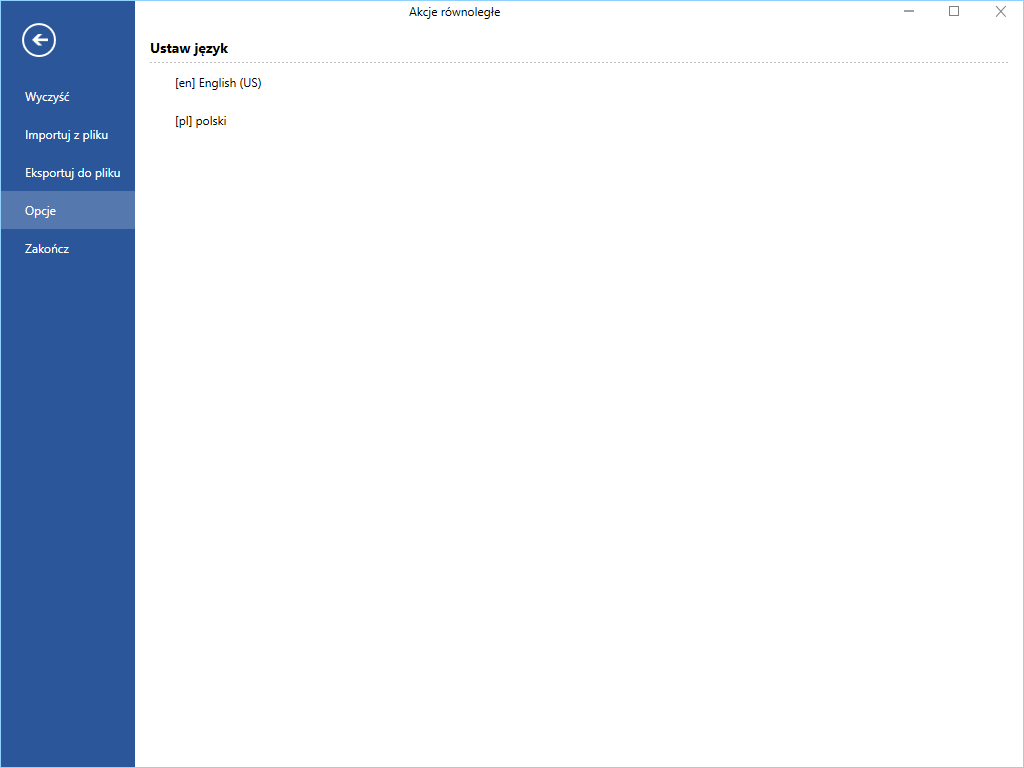
\includegraphics[width=0.8\textwidth]{res/img/options.png}
    \label{fig:options}
    \caption{Menu opcji programu}
\end{figure}

\section{Raport z~przeprowadzonych testów}
\label{sec:our-tests-report}

Zadaniem zespołu było przetestowanie aplikacji opracowanej przez~grupę nr~3.
Tematem projektu nr~3 były \textbf{programy działań w~środowisku wieloagentowym}.

Zespół nr~3 przekazał wersję aplikacji do~testów 4~czerwca.
W~trakcie analizy dokumentacji i~programu wyszczególnione zostały następujące uwagi:

\begin{itemize}
    \item \textbf{Edytor czasem nie wprowadza zmian w~formułach i~kwerendach} \\
    Po~użyciu przycisku do~edycji zdań w~scenariuszu pojawia~się okno dialogowe pozwalające na~zmianę zawartości zdania.
    Po~wprowadzeniu żądanych zmian i~wciśnięciu \emph{Ok} zmiany nie~pojawiają~się w~głównym oknie aplikacji.
    Przy ponownej próbie edycji tego samego zdania wprowadzone zmiany są~jednak widoczne.

    Wciśnięcie przycisku odświeżania po~prawej stronie opcji \emph{Result} w~oknie dialogowym powoduje, że~wprowadzone zmiany są~widoczne wszędzie, lecz naszym zdaniem nie~jest intuicyjne.
    \item \textbf{Awaria aplikacji po~usunięciu wszystkich fluentów i~agentów} \\
    Po~usunięciu wszystkich fluentów i~agentów ze~scenariusza i~wciśnięciu przycisku \emph{Compute} program niespodziewanie się wyłącza.
    \item \textbf{Nazwy fluentów, akcji i~agentów nie~są~unikalne, powodują awarię aplikacji} \\
    Możliwe jest dodanie fluentu, akcji i~agenta o~tej samej nazwie, co~jeden z~istniejących.
    Po~dodaniu duplikatu i~wciśnięciu przycisku \emph{Compute} program niespodziewanie się wyłącza.
    \item \textbf{Błędny wynik zapytania w~historyjce 1. w~porównaniu z~wynikiem w~dokumentacji} \\
    W historyjce 1, w dokumentacji zapytanie: 
    $$\textbf{necessary accessible} \; (M_l) \; \textbf{from} \; (\neg M_l) \; \textbf{by} \; {M}$$
    ma wynik \textsc{False}, podczas gdy w~programie zwrócone jest \textsc{True}, mimo że formuły w~dokumentacji i~programie są~takie same dla~historyjki~1.
    \item \textbf{Awaria aplikacji po~zmianie typu istniejącej kwerendy} \\
    Przy~edycji dowolnej kwerendy, zmiana jej~typu, wciśnięcie \emph{Ok}, a~następnie \emph{Compute} powoduje nieoczekiwany błąd programu.
    \item \textbf{Błędne wyniki kwerend po~modyfikacji historii~1.} \\
    Jeśli po~załadowaniu w~programie historii~1. usuniemy zdanie
    $$\textsc{Attack} \; \textbf{by} \; (M) \; \textbf{releases} \; S_i \; \textbf{if} \; (M_l, S_i) $$
    zmienimy formułę $ \textbf{initially} \; S_i $ na $ \textbf{initially} \; \neg S_i $ i~wciśniemy \emph{Compute}, to~zapytanie
    $$ \textbf{possibly} \; \neg S_i \; \textbf{after} \; (\textsc{Attack} \; \textbf{by} \; (M)) \; \textbf{from} \; (M_i) $$
    zwróci wynik \textsc{False}, chociaż oczekiwany jest wynik \textsc{True}, ponieważ $S_i$ ma~wartość początkową \textsc{False}.
    Natomiast wstawienie zapytania
    $$ \textbf{necessary} \; \neg S_i \; \textbf{after} \; (\textsc{Attack} \; \textbf{by} \; (M)) \; \textbf{from} \; (M_i) $$
    powoduje nieoczekiwane zakończenie programu.
    \item \textbf{Sprzeczne definicje prawdziwości zdania impossible} \\
    Na~stronie~5. dokumentacji dana jest definicja prawdziwości zdania \textbf{impossible}:

    \framebox[\textwidth]{
        \begin{minipage}{0.8\textwidth}
            Wyrażenie $(\textbf{impossible} \; A \; \textbf{by} \; G \; \textbf{if} \; \pi)$ jest prawdziwe w~$S$ wtedy i~tylko wtedy, gdy
            \begin{equation*}
                \forall \sigma \models \pi \rightarrow Res(A, G, \sigma) = \{ \sigma \}
            \end{equation*}
        \end{minipage}
    }

    Natomiast ponieważ zdanie
    $$\textbf{impossible} \; A \; \textbf{by} \; G \; \textbf{if} \; \pi$$
    jest alternatywnym zapisem zdania
    $$A \; \textbf{by} \; G \; \textbf{causes} \; \bot \; \textbf{if} \; \pi$$
    to z~definicji funkcji ${Res}_0$ wynika, że~dla~akcji $A$ objętej zdaniem \textbf{impossible}, pod~warunkiem spełnienia warunku wstępnego~$\pi$, dla~dowolnego stanu $\sigma'$ następnik implikacji w~definicji ${Res}_0$ jest fałszywy, zatem
    $${Res}_0(A,G,\sigma') = Res(A,G,\sigma') = \emptyset$$
    \item \textbf{Historia 2. --- wynik sprzeczny z~grafem przejść w~dokumentacji} \\
    Dla~przykładu~2. (sekcja~4. w~dokumentacji) graf funkcji przejścia przedstawiony w~podsekcji~4.7. pokazuje, że ze~stanu $(L, P)$ nie~powinno być możliwe osiągnięcie stanu $(\neg L, P)$ Tymczasem wprowadzenie do~programu kwerend postaci
    $$ \textbf{possibly accessible} \; (\neg L, P) \; \textbf{from} \; (L, P) \; \textbf{by} \; \{ J \} $$
    $$ \textbf{necessary accessible} \; (\neg L, P) \; \textbf{from} \; (L, P) \; \textbf{by} \; \{ J \} $$
    powoduje uzyskanie dwóch wyników \textsc{True}.
    \item \textbf{Edytor scenariusza nie~pozwala na~wprowadzenie dowolnej formuły} \\
    Dokumentacja specyfikuje, że w zdaniach wartości, obserwacji, ograniczeń i efektu można wstawiać formuły logiczne.
    Edytor zdań scenariusza pozwala jednak tylko na wstawianie literałów.
    \item \textbf{Brak opisu fluentu, akcji lub agenta powoduje awarię aplikacji} \\
    Usunięcie wszystkich agentów, formuł i~akcji, dodanie nowych bez~opisu, a~następnie naciśnięcie przycisku \emph{Compute} program niespodziewanie~się wyłącza.
\end{itemize}

\section{Zgłoszone błędy w~aplikacji}

Stworzona aplikacja dotycząca akcji współbieżnych została przekazana do~testów zespołowi nr~5 26~maja.
Poniżej znajduje~się podsumowanie zgłoszonych błędów wraz~z~opisem sposobu ich~rozwiązania.

\begin{itemize}
    \item \textbf{Dodanie niezależnego nieinercjalnego fluentu zmienia wynik kwerendy}
    \begin{itemize}
        \item \textbf{Opis:}
        Dodanie zdania $\Noninertial c$ do~domeny akcji
        \begin{align*}
            & \textsc{doA} \Causes a \If b \\
            & \Initially \neg a \\
            & \textsc{doB} \Releases b
        \end{align*}
        zmienia wynik kwerendy $\Accessible a$ z~\textsc{True} na~\textsc{False}.
        \item \textbf{Sposób rozwiązania:}
        Podczas analizy błędu okazało~się, że~sposób ewaluacji kwerendy $\Accessible$ był niezgodny z~opisem teoretycznym, ponieważ dla~danego stanu sprawdzane było, czy ze~wszystkich możliwych stanów wynikowych można osiągnąć cel $\gamma$ (zamiast czy można ten cel osiągnąć z~pewnego jednego stanu wynikowego).

        Błąd został naprawiony.
    \end{itemize}
    \item \textbf{Długotrwałe obliczenia}
    \begin{itemize}
        \item \textbf{Opis:}
        Dla~większych sygnatur języka (złożonych z~5~akcji i~3~fluentów) ewaluacja kwerendy typu
        $$ \Accessible \bot $$
        trwa długo (ponad~5~minut)
        \item \textbf{Sposób rozwiązania:}
        Zdaniem zespołu przyczyną jest wykładnicza złożoność znajdowania odpowiedzi na~kwerendy.
        Dla~5~akcji atomowych i~3~fluentów otrzymujemy $2^5 = 32$~akcje złożone i~$2^3 = 8$~fluentów.
        Ponieważ kwerendy typu $\Accessible \bot$ wymagają przejrzenia wszystkich możliwych kombinacji stanów i~akcji, ewaluacja kwerendy sprowadza~się do~rekurencji o~głębokości~8 i~stopniu rozgałęzienia 32.

        Uznajemy, że program działa prawidłowo.
        Do~aplikacji została jednak dodana opcja anulowania trwających obliczeń w~przypadku długotrwałego oczekiwania na~wynik.
    \end{itemize}
\end{itemize}

\section{Podział prac}

W~implementacji aplikacji brali udział wszyscy członkowie zespołu.
Poniżej znajduje~się szczegółowy opis podziału prac w~fazie implementacyjnej.

\begin{itemize}
    \item \textbf{Bartłomiej Dach} przygotował model danych aplikacji.
    \item \textbf{Tymon Felski} i~\textbf{Bartłomiej Dach} przygotowali interfejs użytkownika.
    \item \textbf{Tymon Felski} i~\textbf{Piotr Piwowarski} opracowali zapisywanie i~wczytywanie scenariuszy z~pliku.
    \item \textbf{Jacek Dziwulski} przygotował komponent generujący zbiór wszystkich możliwych stanów oraz zbiór wszystkich akcji złożonych.
    \item \textbf{Maciej Grzeszczak} przygotował część systemu sprowadzającą formuły logiczne do~dysjunkcyjnej postaci normalnej oraz~opracował gramatykę bezkontekstową dla~języka~akcji i~kwerend w~postaci rozszerzonej notacji Backusa-Naura (ang. EBNF --- \emph{Extended Backus-Naur Form}).
    \item \textbf{Filip Grajek} przygotował komponent obliczający dekompozycje poszczególnych akcji złożonych.
    \item \textbf{Piotr Wolski} przygotował komponent wyznaczający wartości funkcji ${Res}_0$.
    \item \textbf{Jędrzej Fijałkowski} przygotował komponent wyznaczający zbiory $New$.
    \item \textbf{Michał Kołodziej} i~\textbf{Mateusz Rymuszka} przygotowali część systemu obliczającą wartości funkcji~$Res$ i~ewaluującą kwerendy.
    \item \textbf{Piotr Piwowarski} przygotował część systemu sprawdzającą prawdziwość zdań wartości i~obserwacji w~domenie akcji.
\end{itemize}

Ponadto \textbf{Bartłomiej Dach}, \textbf{Piotr Wolski}, \textbf{Michał Kołodziej} i~\textbf{Jacek Dziwulski} brali udział w~testach aplikacji zespołu nr~3, których wynikiem były uwagi zawarte w~rozdziale \ref{sec:our-tests-report}.

\section{Opis zawartości płyty~CD}

Płyta~CD dołączona do~raportu zawiera następujące foldery:

\begin{itemize}
    \item Folder \verb+bin/+ zawiera gotową wykonywalną wersję aplikacji.
    Aby uruchomić program, należy wybrać plik \verb+bin/ConcurrentActions.exe+.
    \item Folder \verb+doc/+ zawiera całość dokumentacji projektowej, tj. podstawy teoretyczne projektu oraz~niniejszy raport z~implementacji.
    \item W~folderze \verb+input/+ znajdują~się przykładowe pliki wejściowe dla~programu, w~formatach \verb+.xml+ oraz~\verb+.txt+.
    \item Katalog \verb+src/+ zawiera kod źródłowy opracowanej aplikacji.
\end{itemize}

\end{document}